\chapter{Amplificador de Potencia (PA)}
\label{chap:pa}

La etapa del Amplificador de Potencia utiliza un transistor NPN BFU590G en configuración de emisor común para amplificar la señal de baja potencia centrada en 1 GHz proveniente del VCO y del acoplador direccional antes de la transmisión. El circuito emplea una red de polarización con choques de RF y capacitores de desacople para mantener una operación estable, junto con redes de adaptación LC sintonizadas tanto en la entrada como en la salida para asegurar la adaptación de impedancia a 50 Ohms y el bloqueo de corriente continua. Esta etapa es crítica para aumentar la amplitud de la señal y lograr el rango de detección necesario, actuando a su vez como un búfer para aislar al oscilador de las variaciones de carga en la antena.

\section{Introducción Teórica}

El diseño de amplificadores de potencia (PA) en el dominio de radiofrecuencia se fundamenta en el compromiso de diseño entre la linealidad de la señal de salida y la eficiencia energética del sistema. La clasificación de las topologías de amplificación (Clases A, B, C, etc.) se define rigurosamente mediante el ángulo de conducción ($\theta_c$), parámetro que determina la fracción del ciclo de la señal de excitación durante la cual el dispositivo activo se encuentra en la región activa.

Para la implementación de este radar, se ha seleccionado una configuración en Clase AB. Esta topología establece un punto de operación (Punto Q) intermedio entre la conducción continua de la Clase A y la conducción de medio ciclo de la Clase B.

\subsection{Análisis del Punto de Operación}

La operación en Clase AB se caracteriza por los siguientes aspectos técnicos:

\begin{itemize}
    \item \textbf{Ángulo de Conducción:} 
    El transistor se polariza con una corriente de colector de reposo ($I_{CQ}$) pequeña pero finita, situando el punto $Q$ ligeramente por encima de la región de corte. Esto resulta en un ángulo de conducción en el intervalo $\pi < \theta_c < 2\pi$ (típicamente entre $180^\circ$ y $220^\circ$).
    
    \item \textbf{Linealidad y Distorsión de Cruce:} 
    La motivación principal para emplear Clase AB sobre la Clase B pura es la mitigación de la \textbf{distorsión de cruce} (\textit{crossover distortion}). En la Clase B ($V_{BE} \approx 0$), la no linealidad intrínseca de la unión base-emisor en torno al umbral de encendido ($V_\gamma \approx \qty{0,7}{\V}$ para Si) genera armónicos de alto orden severos cuando la señal cruza por cero. La polarización de la Clase AB linealiza la función de transferencia en esta región crítica, reduciendo significativamente el contenido espectral espurio.

    \item \textbf{Eficiencia de Conversión:} 
    Si bien la eficiencia teórica máxima de la Clase AB es inferior al límite ideal de la Clase B ($\eta_{max} \approx \qty{78,5}{\percent}$), es sustancialmente superior a la de la Clase A ($\eta_{max} = \qty{50}{\percent}$ con carga inductiva, típicamente $<\qty{25}{\percent}$ real). Esto permite manejar potencias de transmisión en el orden de vatios sin los requerimientos térmicos masivos de la Clase A.
\end{itemize}

Para este sistema, la Clase AB asegura que la señal modulada (FMCW) sea amplificada con una fidelidad suficiente para evitar la generación de productos de intermodulación que podrían elevar el piso de ruido del radar, manteniendo simultáneamente un consumo de corriente admisible para la fuente de alimentación.

\section{Desarrollo}

\subsection{Requerimientos de la Etapa}

El diseño del Amplificador de Potencia debe cumplir con los siguientes requerimientos para asegurar su correcto funcionamiento dentro del sistema radar FMCW:

\begin{itemize}
    \item \textbf{Frecuencia central:} El diseño debe estar centrado a una frecuencia de \qty{1}{\GHz}.
    
    \item \textbf{Ancho de banda:} La etapa debe adaptar un ancho de banda de \qty{50}{\MHz} (de \qty{975}{\MHz} a \qty{1025}{\MHz}).
    
    \item \textbf{Adaptación de impedancia (S11):} 
    \begin{itemize}
        \item El parámetro $S_{11}$ debe ser menor o igual a \qty{-10}{\dB} dentro de toda la banda de paso.
        \item En la frecuencia central (\qty{1}{\GHz}), el parámetro $S_{11}$ debe ser menor o igual a \qty{-20}{\dB}.
    \end{itemize}
    
    \item \textbf{Ganancia (S21):} La ganancia de la etapa a la frecuencia central debe encontrarse dentro de un rango de \qty{12}{\dB} a \qty{15}{\dB}, debido a las limitaciones inherentes del transistor BFU590G.
\end{itemize}

\subsection{Diseño de Referencia}

El diseño del Amplificador de Potencia se basa en la nota de aplicación AN11501 de NXP Semiconductors \cite{nxp_an11501}, la cual proporciona una guía técnica completa para el diseño de un PA para la banda ISM de 866 MHz utilizando el transistor de banda ancha BFU590G. Este documento sirve como punto de partida para el diseño.

La arquitectura propuesta en la nota de aplicación consiste en un amplificador de emisor común de una sola etapa, operando en Clase AB. Los aspectos principales del diseño de referencia son:

\begin{itemize}
    \item \textbf{Componente activo:} Transistor NPN de banda ancha BFU590G con emisor conectado directamente a tierra para maximizar la ganancia de potencia.
    
    \item \textbf{Red de entrada:} Incluye un capacitor de bloqueo de CC (\qty{100}{\pF}), una red de adaptación LC (\qty{3,3}{\pF} y \qty{1,5}{\nH}) para transformar la impedancia de entrada a \qty{50}{\ohm}, y choques de RF (inductores de \qty{470}{\nH}) para aislar la fuente de polarización de la señal de RF.
    
    \item \textbf{Red de salida:} Comprende un RFC (Radio Frequency Choke) de \qty{18}{\nH} para suministrar continua al colector mientras presenta alta impedancia a la RF, junto con una red de adaptación (\qty{6,8}{\nH}) y capacitor de bloqueo de continua (\qty{100}{\pF}) en la salida.
    
    \item \textbf{Polarización:} Voltaje de alimentación $V_{cc} = \qty{8}{\V}$ con capacitores de desacople (\qty{22}{\nF} y \qty{100}{\pF}) para filtrar ruido.
\end{itemize}

La Figura \ref{fig:pa_reference_schematic} muestra el esquemático del diseño de referencia extraído de la nota de aplicación.

\begin{figure}[htbp]
\centering
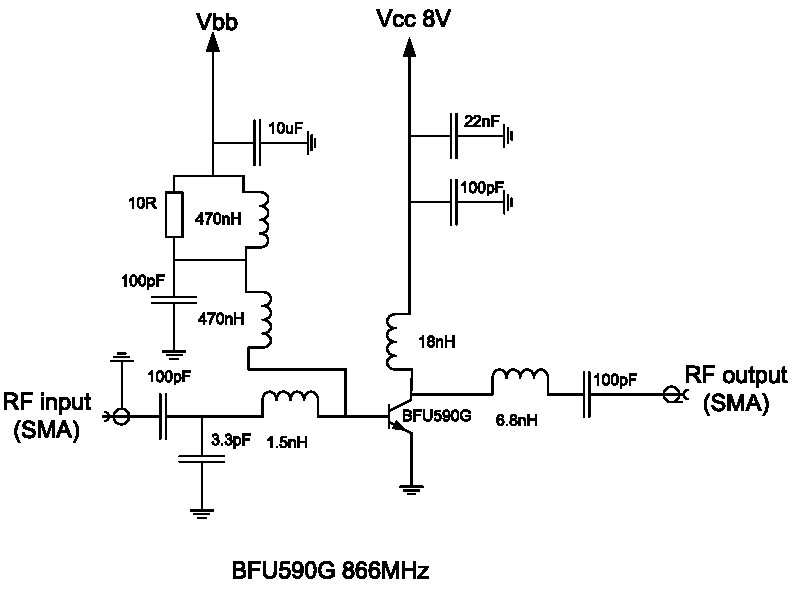
\includegraphics[width=0.9\textwidth]{Figures/2_PA/BFU590G_REFERENCE.pdf}
\captionsetup{justification=centering}
\caption{Esquemático del PA de referencia para \\ 866 MHz con transistor BFU590G \cite{nxp_an11501}.}
\label{fig:pa_reference_schematic}
\end{figure}


Los resultados reportados en la nota de aplicación para el diseño a \qty{866}{\MHz} incluyen: potencia de salida P1dB de \qty{27}{\dBm}, eficiencia del \qty{55}{\percent}, y ganancia de \qty{10}{\dB}. El documento también indica que el diseño puede sintonizarse a otras frecuencias modificando los valores de los componentes en las redes de adaptación.

Para adaptar este diseño de referencia a la frecuencia central de \qty{1}{\GHz}, requerida por el radar, se redefinirán los valores de algunos componentes utilizando la herramienta de optimización.

\subsection{Incorporación del BFU590G a la Librería del Proyecto}

Para incluir el transistor BFU590G en el entorno de simulación, se incorporó al proyecto de Keysight ADS el design kit \texttt{BFU5XX\_FAMILY\_ADS\_DESIGN\_KIT\_V2}, disponible en la página del fabricante NXP\footnote{\url{https://www.nxp.com/products/radio-frequency-rf/legacy-rf/legacy-rf-wideband-transistors/npn-wideband-silicon-rf-transistor:BFU590}}.

Una vez instalado el design kit, se utilizó la plantilla de test bench \texttt{BJT\_curve\_tracer} disponible por defecto en ADS para verificar el comportamiento del transistor. La Figura \ref{fig:bfu590g_testbench} muestra el esquema de simulación configurado para obtener las curvas características del dispositivo.

\begin{figure}[htbp]
\centering
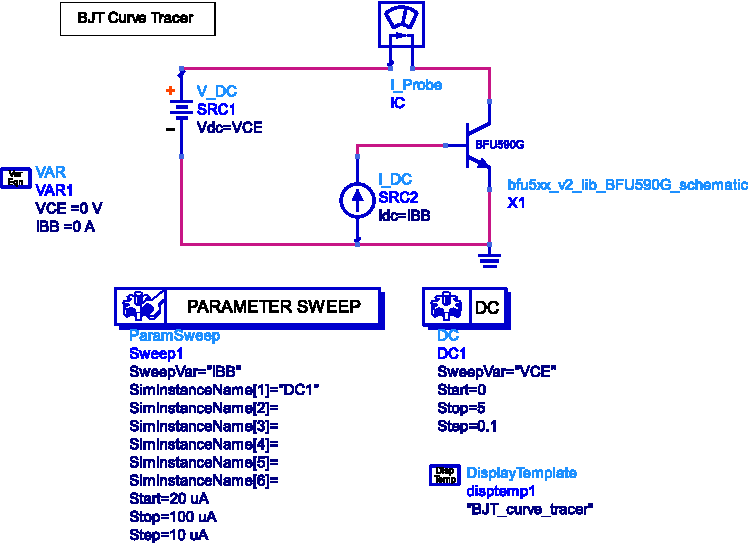
\includegraphics[width=0.85\textwidth]{Figures/2_PA/BFU590G_TEST_BENCH_ADS.pdf}
\captionsetup{justification=centering}
\caption{Esquema de simulación del test bench \texttt{BJT\_curve\_tracer} \\ para el transistor BFU590G.}
\label{fig:bfu590g_testbench}
\end{figure}

El circuito consiste en el transistor en configuración de emisor común, con una fuente de voltaje que varía $V_{CE}$ de \qty{0}{\V} a \qty{5}{\V} en pasos de \qty{0,1}{\V}, y un barrido paramétrico de la corriente de base $I_{BB}$ desde \qty{20}{\uA} hasta \qty{100}{\uA} en incrementos de \qty{10}{\uA}.

Los resultados de la simulación se presentan en la Figura \ref{fig:bfu590g_results}, donde se observan las curvas de corriente de colector $I_C$ en función del voltaje $V_{CE}$ para cada nivel de corriente de base. El marcador indica un punto de operación representativo en $V_{CE} = \qty{3}{\V}$ e $I_C = \qty{6}{\mA}$, con un consumo de potencia de aproximadamente \qty{17}{\mW}.

\begin{figure}[htbp]
\centering
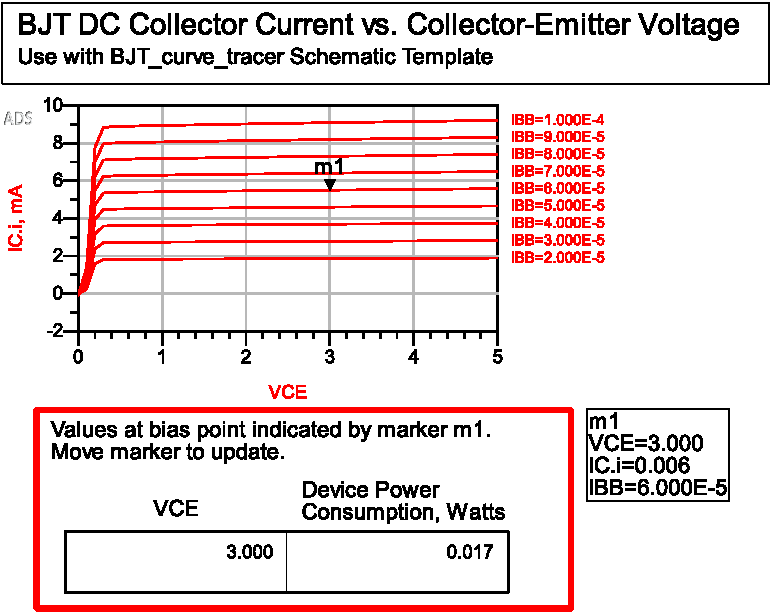
\includegraphics[width=0.7\textwidth]{Figures/2_PA/BFU590G_TEST_BENCH_RESULTS_ADS.pdf}
\captionsetup{justification=centering}
\caption{Curvas características $I_C$ vs. $V_{CE}$ del transistor BFU590G \\ obtenidas mediante el test bench.}
\label{fig:bfu590g_results}
\end{figure}

\subsection{Implementación del Circuito Parametrizado}

Con el objetivo de facilitar el proceso de optimización y prueba del diseño, se implementó el amplificador de potencia como un componente jerárquico reutilizable en ADS, denominado \texttt{pa\_core}. Este enfoque permite encapsular el circuito completo en un símbolo de bloque con parámetros configurables, posibilitando modificar valores críticos sin alterar el esquemático interno.

La Figura \ref{fig:pa_core_diagram} muestra el diagrama del circuito parametrizado, donde se observa el símbolo jerárquico junto con su esquemático interno detallado. El componente cuenta con dos terminales: P1 (entrada) y P2 (salida), ambos adaptados a $50\,\Omega$.

\begin{figure}[!htb]
\centering
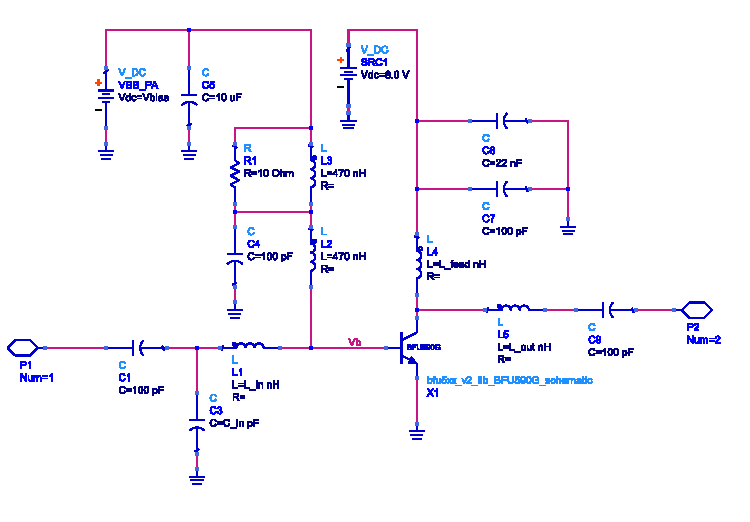
\includegraphics[width=0.8\textwidth]{Figures/2_PA/PA_CORE_circuit_diagram.pdf}
\captionsetup{justification=centering}
\caption{Diagrama del componente \texttt{pa\_core}: símbolo jerárquico \\ y esquemático interno parametrizado.}
\label{fig:pa_core_diagram}
\end{figure}

El esquemático interno implementa la topología del diseño de referencia AN11501, incorporando:

\begin{itemize}
    \item \textbf{Red de entrada:} Capacitor de bloqueo DC (100 pF), seguido de una red de adaptación LC con valores parametrizados.
    
    \item \textbf{Red de polarización:} Fuente de tensión configurable para la base, con choques de RF (470 nH) y capacitores de desacoplo para estabilidad.
    
    \item \textbf{Red de salida:} Inductor de alimentación (RFC) parametrizado, red de adaptación y capacitor de bloqueo DC (100 pF).
    
    \item \textbf{Alimentación:} Voltaje de colector fijo de $V_{CC} = 8\,\text{V}$ con filtrado adecuado.
\end{itemize}

La Tabla \ref{tab:pa_core_params} resume los parámetros configurables del componente y sus valores iniciales, extraídos del diseño de referencia para \qty{866}{\MHz}. Estos valores servirán como punto de partida para la optimización a \qty{1}{\GHz}.

\begin{table}[!htb]
\centering
\small
\caption{Parámetros configurables del componente \texttt{pa\_core}.}
\label{tab:pa_core_params}
\begin{tabular}{@{}llcl@{}}
\toprule
\textbf{Parámetro} & \textbf{Descripción} & \textbf{Valor} & \textbf{Unidad} \\
\midrule
\texttt{Vbias}   & Voltaje de polarización de base   & 0.8  & V  \\
\texttt{C\_in}   & Capacitor de adaptación de entrada & 3.3  & pF \\
\texttt{L\_in}   & Inductor de adaptación de entrada  & 1.5  & nH \\
\texttt{L\_feed} & Inductor de alimentación (RFC)     & 18   & nH \\
\texttt{L\_out}  & Inductor de adaptación de salida   & 6.8  & nH \\
\bottomrule
\end{tabular}
\end{table}

El valor de \texttt{Vbias} se establece inicialmente en \qty{0,8}{\V} para situar el transistor en Clase AB, y será ajustado posteriormente mediante optimización para obtener el punto de operación óptimo. Los valores de los componentes reactivos (\texttt{C\_in}, \texttt{L\_in}, \texttt{L\_feed}, \texttt{L\_out}) corresponden al diseño de \qty{866}{\MHz} y serán reoptimizados para la frecuencia central de \qty{1}{\GHz}.

\subsection{Optimización de Componentes para Frecuencia Central de 1 GHz}

Una vez obtenido el componente parametrizado de la etapa se procede con el proceso de optimización de los valores del circuito para satisfacer los requerimientos mencionados anteriormente. A diferencia de un diseño manual, en esta etapa se utiliza el software ADS para encontrar automáticamente los valores ideales de los componentes que cumplan con las metas de rendimiento especificadas.

\subsubsection{Configuración de la Optimización}

La Figura \ref{fig:pa_opt_circuit} muestra el esquemático de simulación configurado para el proceso de optimización, donde se definen las metas de rendimiento y los parámetros del algoritmo.

\begin{figure}[htbp]
\centering
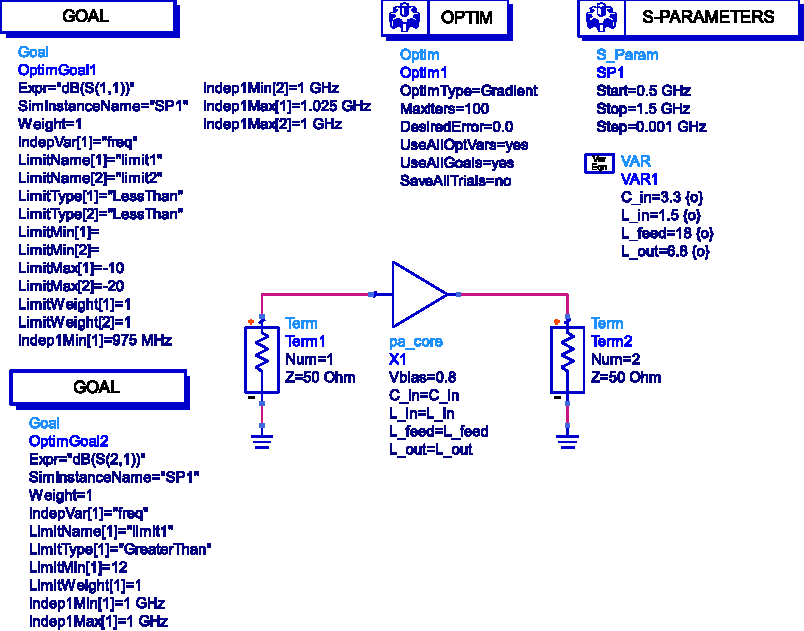
\includegraphics[width=0.7\textwidth]{Figures/2_PA/PA_BANDWIDTH_OPT_circuit.pdf}
\captionsetup{justification=centering}
\caption{Configuración de optimización del PA en ADS: \\ metas de rendimiento y parámetros del algoritmo.}
\label{fig:pa_opt_circuit}
\end{figure}

El esquemático incluye los siguientes bloques de configuración:

\begin{itemize}
    \item \textbf{Bloque OPTIM:} Utiliza un algoritmo de tipo \textit{Gradient} (Gradiente), configurado para realizar un máximo de 100 iteraciones.
    
    \item \textbf{Bloque S-PARAMETERS:} Define el rango de frecuencia de barrido desde \qty{0,5}{\GHz} hasta \qty{1,5}{\GHz}.
    
    \item \textbf{Goal 1 ($S_{11}$):} Define las metas para la adaptación de entrada:
    \begin{itemize}
        \item $S_{11} \leq \qty{-10}{\dB}$ en el rango de \qty{975}{\MHz} a \qty{1025}{\MHz}.
        \item $S_{11} \leq \qty{-20}{\dB}$ a la frecuencia central de \qty{1}{\GHz}.
    \end{itemize}
    
    \item \textbf{Goal 2 ($S_{21}$):} Define la meta para la ganancia: $S_{21} \geq \qty{12}{\dB}$ a \qty{1}{\GHz}.
\end{itemize}

Los parámetros habilitados para optimización son \texttt{C\_in}, \texttt{L\_in}, \texttt{L\_feed} y \texttt{L\_out}, identificados con la marca \texttt{\{o\}} en el bloque de variables.

\subsubsection{Resultados de la Optimización}

La Figura \ref{fig:pa_opt_cockpit} muestra el panel de control (\textit{Optimization Cockpit}) de ADS al finalizar el proceso de optimización.

\begin{figure}[htbp]
\centering
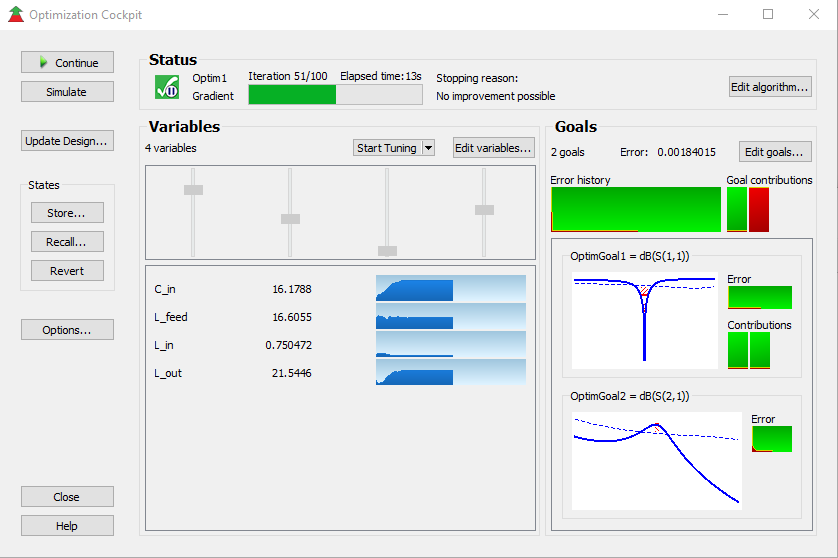
\includegraphics[width=0.85\textwidth]{Figures/2_PA/pa_optimizer_bandwidth_cockpit.png}
\captionsetup{justification=centering}
\caption{Panel de control de optimización mostrando la convergencia del algoritmo.}
\label{fig:pa_opt_cockpit}
\end{figure}

El proceso de optimización se detuvo en la \textbf{iteración 51 de 100} debido a que el algoritmo detectó que no era posible mejorar más los resultados (se alcanzó el punto óptimo). Las gráficas en el panel muestran:

\begin{itemize}
    \item La evolución de las variables optimizadas hasta estabilizarse en sus valores finales.
    \item El cumplimiento de las metas de $S_{11}$ (caída pronunciada a 1 GHz) y $S_{21}$ (pico de ganancia).
    \item El error residual cercano a cero, indicando que todas las metas fueron satisfechas.
\end{itemize}

\subsubsection{Comparación de Resultados: Antes y Después}

Las siguientes figuras comparan el comportamiento del amplificador con los valores originales de 866 MHz (línea punteada) y los valores optimizados para 1 GHz (línea sólida).

\begin{figure}[htbp]
\centering
\begin{tikzpicture}
\begin{axis}[
    width=0.9\textwidth,
    height=7cm,
    xlabel={Frecuencia [GHz]},
    ylabel={$S_{11}$ [dB]},
    xmin=0.5, xmax=1.5,
    ymin=-55, ymax=0,
    grid=both,
    grid style={line width=.1pt, draw=gray!30},
    major grid style={line width=.2pt,draw=gray!50},
    legend pos=south east,
    legend style={font=\footnotesize},
    tick label style={font=\footnotesize},
    label style={font=\small},
]
% Datos antes de optimización (866 MHz)
\addplot[blue, dashed, thick] table[
    x expr=\thisrowno{0}/1e9,
    y expr=\thisrowno{1},
    col sep=tab,
    skip first n=1
] {Datasets/2_PA/data_optimization_pa_core_s11_866MHZ.dat};
\addlegendentry{Original (866 MHz)}

% Datos después de optimización (1 GHz)
\addplot[red, thick] table[
    x expr=\thisrowno{1}/1e9,
    y expr=\thisrowno{2},
    col sep=tab,
    skip first n=1
] {Datasets/2_PA/data_optimization_pa_core_s11_1GHZ.dat};
\addlegendentry{Optimizado (1 GHz)}

% Línea de referencia -10 dB
\addplot[black, dashed, line width=0.8pt] coordinates {(0.5,-10) (1.5,-10)};
\node[anchor=south west, font=\scriptsize, fill=white, inner sep=1pt] at (axis cs:0.52,-10) {$-10$ dB};

% Línea de referencia -20 dB
\addplot[black, dashed, line width=0.8pt] coordinates {(0.5,-20) (1.5,-20)};
\node[anchor=south west, font=\scriptsize, fill=white, inner sep=1pt] at (axis cs:0.52,-20) {$-20$ dB};

\end{axis}
\end{tikzpicture}
\captionsetup{justification=centering}
\caption{Comparación de $S_{11}$ antes y después de la optimización.}
\label{fig:pa_s11_comparison}
\end{figure}

La Figura \ref{fig:pa_s11_comparison} evidencia la resintonización del amplificador. Con los valores originales, el parámetro $S_{11}$ presenta valores relativamente constantes alrededor de \qty{-3}{\dB} a \qty{-6}{\dB} en todo el rango, sin un punto de adaptación definido. Tras la optimización, se observa una pronunciada caída de $S_{11}$ centrada en \qty{1}{\GHz}, alcanzando valores inferiores a \qty{-50}{\dB} en la frecuencia central y cumpliendo holgadamente el requisito de \qty{-20}{\dB}.

\begin{figure}[htbp]
\centering
\begin{tikzpicture}
\begin{axis}[
    width=0.9\textwidth,
    height=7cm,
    xlabel={Frecuencia [GHz]},
    ylabel={$S_{21}$ [dB]},
    xmin=0.5, xmax=1.5,
    ymin=0, ymax=16,
    grid=both,
    grid style={line width=.1pt, draw=gray!30},
    major grid style={line width=.2pt,draw=gray!50},
    legend pos=south west,
    legend style={font=\footnotesize},
    tick label style={font=\footnotesize},
    label style={font=\small},
]
% Datos antes de optimización (866 MHz)
\addplot[blue, dashed, thick] table[
    x expr=\thisrowno{0}/1e9,
    y expr=\thisrowno{1},
    col sep=tab,
    skip first n=1
] {Datasets/2_PA/data_optimization_pa_core_s21_866MHZ.dat};
\addlegendentry{Original (866 MHz)}

% Datos después de optimización (1 GHz)
\addplot[red, thick] table[
    x expr=\thisrowno{1}/1e9,
    y expr=\thisrowno{2},
    col sep=tab,
    skip first n=1
] {Datasets/2_PA/data_optimization_pa_core_s21_1GHZ.dat};
\addlegendentry{Optimizado (1 GHz)}

% Línea de referencia 12 dB
\addplot[black, dashed, line width=0.8pt] coordinates {(0.5,12) (1.5,12)};
\node[anchor=south west, font=\scriptsize, fill=white, inner sep=1pt] at (axis cs:0.52,12) {$12$ dB};

\end{axis}
\end{tikzpicture}
\captionsetup{justification=centering}
\caption{Comparación de $S_{21}$ antes y después de la optimización.}
\label{fig:pa_s21_comparison}
\end{figure}

La Figura \ref{fig:pa_s21_comparison} muestra la respuesta de ganancia del amplificador. Con los valores originales diseñados para \qty{866}{\MHz}, la ganancia presenta una respuesta decreciente con la frecuencia, iniciando en aproximadamente \qty{13}{\dB} a \qty{500}{\MHz} y cayendo progresivamente. Después de la optimización, la ganancia muestra un pico pronunciado centrado en \qty{1}{\GHz}, alcanzando aproximadamente $\mathbf{\qty{11,5}{\dB}}$ en la frecuencia central, valor cercano al objetivo de \qty{12}{\dB}.

\subsubsection{Valores Optimizados de los Componentes}

La Tabla \ref{tab:pa_opt_values} resume los valores de los componentes antes y después del proceso de optimización.

\begin{table}[htbp]
\centering
\small
\caption{Valores optimizados y componentes comerciales seleccionados.}
\label{tab:pa_opt_values}
\begin{tabular}{@{}lcccl@{}}
\toprule
\textbf{Parámetro} & \textbf{Original} & \textbf{Optimizado} & \textbf{Comercial} & \textbf{Unidad} \\
\midrule
\texttt{C\_in}   & 3.3   & 16.17  & 16    & pF \\
\texttt{L\_in}   & 1.5   & 0.75   & 0.75  & nH \\
\texttt{L\_feed} & 18    & 16.60  & 16    & nH \\
\texttt{L\_out}  & 6.8   & 21.54  & 22    & nH \\
\bottomrule
\end{tabular}
\end{table}

El proceso de optimización permite adaptar exitosamente el diseño de referencia de \qty{866}{\MHz} a la frecuencia central de \qty{1}{\GHz} requerida por el sistema radar, cumpliendo con los objetivos de adaptación de entrada ($S_{11} < \qty{-20}{\dB}$ a \qty{1}{\GHz}) y aproximándose al objetivo de ganancia ($S_{21} \approx \qty{12}{\dB}$).

\subsection{Optimización de Tensión de Polarización}

Mientras que en la etapa anterior se optimizaron los componentes pasivos ($L$ y $C$), en esta fase el objetivo es encontrar el voltaje de base (\textbf{Vbias}) ideal para maximizar la ganancia en condiciones no lineales. Para ello se utiliza una simulación de \textbf{Balance Armónico} (\textit{Harmonic Balance}), técnica que permite analizar el comportamiento real del transistor cuando se le inyecta una señal de potencia.

\subsubsection{Configuración de la Simulación No Lineal}

La Figura \ref{fig:pa_vbias_circuit} muestra el esquema de simulación configurado para la optimización del punto de polarización.

\begin{figure}[htbp]
\centering
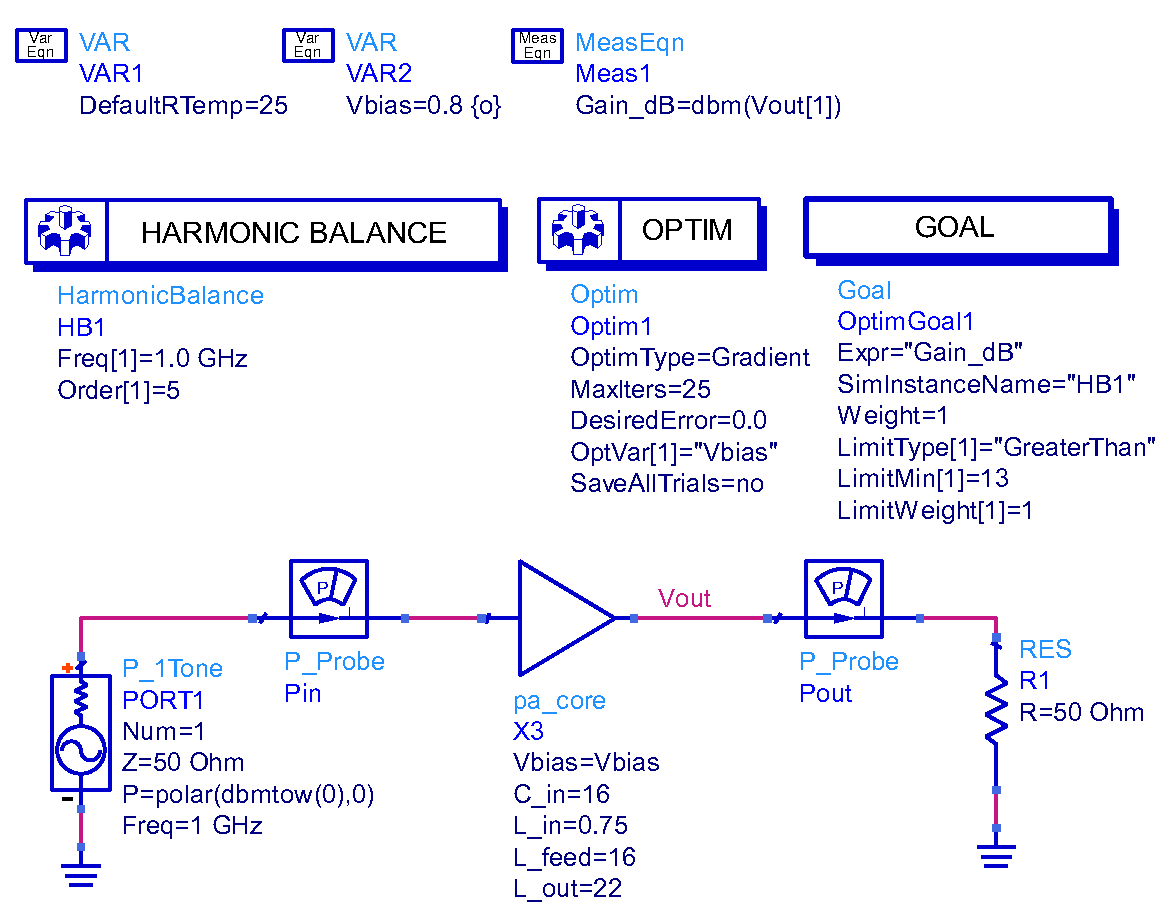
\includegraphics[width=0.8\textwidth]{Figures/2_PA/PA_VBIAS_OPTIMIZATION_circuit.pdf}
\captionsetup{justification=centering}
\caption{Esquema de simulación de Balance Armónico para \\ la optimización del voltaje de polarización.}
\label{fig:pa_vbias_circuit}
\end{figure}

El esquemático incluye los siguientes bloques de configuración:

\begin{itemize}
    \item \textbf{Bloque HARMONIC BALANCE (HB1):} A diferencia de los parámetros S (que son lineales), el Balance Armónico analiza la distorsión y el comportamiento no lineal a \qty{1,0}{\GHz}. Se ha configurado con un orden de 5 para capturar los armónicos.
    
    \item \textbf{Bloque OPTIM:} Configurado para optimizar específicamente la variable \texttt{Vbias}, utilizando el algoritmo de Gradiente con un máximo de 25 iteraciones.
    
    \item \textbf{Bloque GOAL (OptimGoal1):} La meta establecida es que la ganancia (\texttt{Gain\_dB}) sea mayor a \qty{13}{\dB}.
    
    \item \textbf{Variables de Circuito:} Los valores de $C\_in$, $L\_in$, $L\_feed$ y $L\_out$ se mantienen fijos en \num{16}, \num{0,75}, \num{16} y \num{22} respectivamente (valores comerciales de la optimización previa).
    
    \item \textbf{Componentes de Medición:} Se utilizan sondas de potencia (\texttt{P\_Probe}) en la entrada (\texttt{Pin}) y salida (\texttt{Pout}) para calcular la ganancia de forma precisa.
\end{itemize}

\subsubsection{Vista General del Barrido de Vbias}

Antes de ejecutar la optimización automática, se realizó un barrido paramétrico de la tensión de polarización para observar la tendencia del comportamiento. La Figura \ref{fig:pa_vbias_sweep} muestra la ganancia en función de \texttt{Vbias} en el rango de \qty{0,7}{\V} a \qty{0,95}{\V}.

\begin{figure}[htbp]
\centering
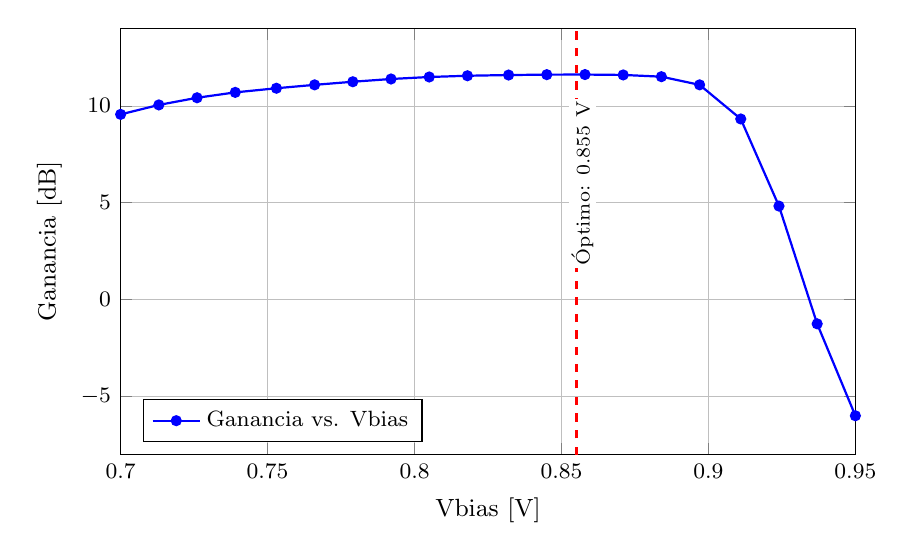
\begin{tikzpicture}
\begin{axis}[
    width=0.9\textwidth,
    height=7cm,
    xlabel={Vbias [V]},
    ylabel={Ganancia [dB]},
    xmin=0.7, xmax=0.95,
    ymin=-8, ymax=14,
    grid=both,
    grid style={line width=.1pt, draw=gray!30},
    major grid style={line width=.2pt,draw=gray!50},
    legend pos=south west,
    legend style={font=\footnotesize},
    tick label style={font=\footnotesize},
    label style={font=\small},
    mark options={scale=0.8},
]
% Datos del barrido de Vbias
\addplot[blue, thick, mark=*] coordinates {
    (0.700, 9.557)
    (0.713, 10.045)
    (0.726, 10.414)
    (0.739, 10.692)
    (0.753, 10.905)
    (0.766, 11.080)
    (0.779, 11.240)
    (0.792, 11.382)
    (0.805, 11.485)
    (0.818, 11.549)
    (0.832, 11.586)
    (0.845, 11.606)
    (0.858, 11.611)
    (0.871, 11.591)
    (0.884, 11.501)
    (0.897, 11.080)
    (0.911, 9.321)
    (0.924, 4.829)
    (0.937, -1.243)
    (0.950, -5.983)
};
\addlegendentry{Ganancia vs. Vbias}

% Línea de referencia del óptimo
\addplot[red, dashed, line width=1pt] coordinates {(0.855,{-8}) (0.855,{14})};
\node[anchor=south, font=\scriptsize, fill=white, inner sep=1pt, rotate=90] at (axis cs:0.862,6) {Óptimo: 0.855 V};

\end{axis}
\end{tikzpicture}
\captionsetup{justification=centering}
\caption{Barrido paramétrico de la ganancia en función de Vbias.}
\label{fig:pa_vbias_sweep}
\end{figure}

Se observa que la ganancia presenta un máximo en torno a \qty{0,855}{\V}, alcanzando aproximadamente \qty{11,6}{\dB}. Para valores de \texttt{Vbias} superiores a \qty{0,9}{\V}, la ganancia cae abruptamente debido a que el transistor entra en una zona de saturación excesiva.

\subsubsection{Resultados de la Optimización}

La Figura \ref{fig:pa_vbias_cockpit} muestra el panel de control de optimización al finalizar el proceso.

\begin{figure}[htbp]
\centering
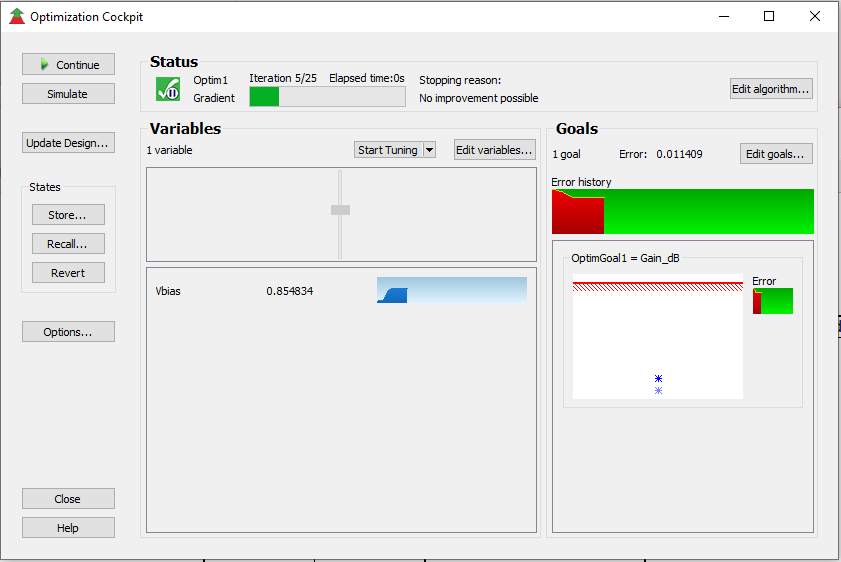
\includegraphics[width=0.85\textwidth]{Figures/2_PA/pa_optimizer_vbias_cockpit.png}
\captionsetup{justification=centering}
\caption{Panel de control de optimización mostrando la convergencia \\ del algoritmo para la optimización de Vbias.}
\label{fig:pa_vbias_cockpit}
\end{figure}

El proceso de optimización se detuvo en la \textbf{iteración 5 de 25} debido a que el algoritmo detectó que se había alcanzado el punto máximo donde ya no era posible mejorar más. El software determinó que el valor ideal para \texttt{Vbias} es:

\begin{equation}
\boxed{V_{bias} = \qty{0,854834}{\V}}
\end{equation}

Este ligero aumento respecto al valor inicial de \qty{0,8}{\V} desplaza al transistor a una zona de mayor conducción, lo que incrementa la ganancia disponible.

\subsubsection{Parámetros S con Valores Finales}

Las siguientes figuras presentan los parámetros S del amplificador con los valores comerciales de componentes optimizados y la tensión de polarización ajustada a \qty{0,854834}{\V}.

\begin{figure}[htbp]
\centering
\begin{tikzpicture}
\begin{axis}[
    width=0.9\textwidth,
    height=7cm,
    xlabel={Frecuencia [GHz]},
    ylabel={$S_{11}$ [dB]},
    xmin=0.5, xmax=1.5,
    ymin=-35, ymax=0,
    grid=both,
    grid style={line width=.1pt, draw=gray!30},
    major grid style={line width=.2pt,draw=gray!50},
    legend pos=south east,
    legend style={font=\footnotesize},
    tick label style={font=\footnotesize},
    label style={font=\small},
]
% Datos de S11 con valores optimizados finales
\addplot[blue, thick] table[
    x expr=\thisrowno{0}/1e9,
    y expr=\thisrowno{1},
    col sep=tab,
    skip first n=1
] {Datasets/2_PA/data_pa_s_parameters_optimized_values_s11.dat};
\addlegendentry{$S_{11}$ Final}

% Línea de referencia -10 dB
\addplot[black, dashed, line width=0.8pt] coordinates {(0.5,-10) (1.5,-10)};
\node[anchor=south west, font=\scriptsize, fill=white, inner sep=1pt] at (axis cs:0.52,-10) {$-10$ dB};

% Línea de referencia -20 dB
\addplot[black, dashed, line width=0.8pt] coordinates {(0.5,-20) (1.5,-20)};
\node[anchor=south west, font=\scriptsize, fill=white, inner sep=1pt] at (axis cs:0.52,-20) {$-20$ dB};

\end{axis}
\end{tikzpicture}
\captionsetup{justification=centering}
\caption{Parámetro $S_{11}$ del PA con valores comerciales y Vbias optimizado.}
\label{fig:pa_s11_final}
\end{figure}

La Figura \ref{fig:pa_s11_final} muestra que el parámetro $S_{11}$ presenta una adaptación óptima centrada en \qty{1}{\GHz}, alcanzando valores inferiores a \qty{-25}{\dB} en la frecuencia central. Dentro de la banda de paso (\qty{975}{\MHz} a \qty{1025}{\MHz}), el $S_{11}$ se mantiene por debajo de \qty{-10}{\dB}, cumpliendo holgadamente el requisito especificado.

\begin{figure}[htbp]
\centering
\begin{tikzpicture}
\begin{axis}[
    width=0.9\textwidth,
    height=7cm,
    xlabel={Frecuencia [GHz]},
    ylabel={$S_{21}$ [dB]},
    xmin=0.5, xmax=1.5,
    ymin=0, ymax=14,
    grid=both,
    grid style={line width=.1pt, draw=gray!30},
    major grid style={line width=.2pt,draw=gray!50},
    legend pos=south west,
    legend style={font=\footnotesize},
    tick label style={font=\footnotesize},
    label style={font=\small},
]
% Datos de S21 con valores optimizados finales
\addplot[blue, thick] table[
    x expr=\thisrowno{0}/1e9,
    y expr=\thisrowno{1},
    col sep=tab,
    skip first n=1
] {Datasets/2_PA/data_pa_s_parameters_optimized_values_s21.dat};
\addlegendentry{$S_{21}$ Final}

% Línea de referencia 12 dB
\addplot[black, dashed, line width=0.8pt] coordinates {(0.5,12) (1.5,12)};
\node[anchor=south west, font=\scriptsize, fill=white, inner sep=1pt] at (axis cs:0.52,12) {$12$ dB};

\end{axis}
\end{tikzpicture}
\captionsetup{justification=centering}
\caption{Parámetro $S_{21}$ del PA con valores comerciales y Vbias optimizado.}
\label{fig:pa_s21_final}
\end{figure}

La Figura \ref{fig:pa_s21_final} muestra la respuesta de ganancia del amplificador optimizado. Se observa un pico de ganancia centrado en \qty{1}{\GHz}, alcanzando aproximadamente $\mathbf{\qty{11,6}{\dB}}$ en la frecuencia central. Este valor se encuentra dentro del rango objetivo de $\qty{12}{\dB}\pm\qty{3}{\dB}$ especificado para la etapa.

\begin{figure}[htbp]
\centering
\begin{tikzpicture}
\begin{axis}[
    width=0.9\textwidth,
    height=7cm,
    xlabel={Frecuencia [GHz]},
    ylabel={$S_{22}$ [dB]},
    xmin=0.5, xmax=1.5,
    ymin=-35, ymax=0,
    grid=both,
    grid style={line width=.1pt, draw=gray!30},
    major grid style={line width=.2pt,draw=gray!50},
    legend pos=south east,
    legend style={font=\footnotesize},
    tick label style={font=\footnotesize},
    label style={font=\small},
]
% Datos de S22 con valores optimizados finales
\addplot[blue, thick] table[
    x expr=\thisrowno{0}/1e9,
    y expr=\thisrowno{1},
    col sep=tab,
    skip first n=1
] {Datasets/2_PA/data_pa_s_parameters_optimized_values_s22.dat};
\addlegendentry{$S_{22}$ Final}

% Línea de referencia -10 dB
\addplot[black, dashed, line width=0.8pt] coordinates {(0.5,-10) (1.5,-10)};
\node[anchor=south west, font=\scriptsize, fill=white, inner sep=1pt] at (axis cs:0.52,-10) {$-10$ dB};

\end{axis}
\end{tikzpicture}
\captionsetup{justification=centering}
\caption{Parámetro $S_{22}$ del PA con valores comerciales y Vbias optimizado.}
\label{fig:pa_s22_final}
\end{figure}

La Figura \ref{fig:pa_s22_final} muestra la adaptación de salida del amplificador. Se observa que el $S_{22}$ alcanza un mínimo pronunciado en torno a \qty{1,01}{\GHz}, con valores inferiores a \qty{-30}{\dB}. Este resultado indica una excelente adaptación en la salida del amplificador.

\begin{figure}[htbp]
\centering
\begin{tikzpicture}
\begin{axis}[
    width=0.9\textwidth,
    height=7cm,
    xlabel={Frecuencia [GHz]},
    ylabel={$S_{12}$ [dB]},
    xmin=0.5, xmax=1.5,
    ymin=-30, ymax=-10,
    grid=both,
    grid style={line width=.1pt, draw=gray!30},
    major grid style={line width=.2pt,draw=gray!50},
    legend pos=south west,
    legend style={font=\footnotesize},
    tick label style={font=\footnotesize},
    label style={font=\small},
]
% Datos de S12 con valores optimizados finales
\addplot[blue, thick] table[
    x expr=\thisrowno{0}/1e9,
    y expr=\thisrowno{1},
    col sep=tab,
    skip first n=1
] {Datasets/2_PA/data_pa_s_parameters_optimized_values_s12.dat};
\addlegendentry{$S_{12}$ Final}

\end{axis}
\end{tikzpicture}
\captionsetup{justification=centering}
\caption{Parámetro $S_{12}$ del PA con valores comerciales y Vbias optimizado.}
\label{fig:pa_s12_final}
\end{figure}

La Figura \ref{fig:pa_s12_final} presenta el aislamiento inverso del amplificador ($S_{12}$). Los valores se mantienen por debajo de \qty{-12}{\dB} en todo el rango de frecuencias, alcanzando un mínimo de aproximadamente \qty{-27}{\dB} en la banda de operación. Este nivel de aislamiento es adecuado para evitar la realimentación de señales desde la salida hacia la entrada.

\subsubsection{Resumen de Valores Finales del Diseño}

La Tabla \ref{tab:pa_final_values} resume los valores finales del amplificador de potencia tras ambos procesos de optimización.

\begin{table}[htbp]
\centering
\small
\caption{Valores finales del diseño del PA optimizado.}
\label{tab:pa_final_values}
\begin{tabular}{@{}lccl@{}}
\toprule
\textbf{Parámetro} & \textbf{Valor Inicial} & \textbf{Valor Final} & \textbf{Unidad} \\
\midrule
\texttt{Vbias}   & 0.800    & 0.855    & V  \\
\texttt{C\_in}   & 3.3      & 16       & pF \\
\texttt{L\_in}   & 1.5      & 0.75     & nH \\
\texttt{L\_feed} & 18       & 16       & nH \\
\texttt{L\_out}  & 6.8      & 22       & nH \\
\bottomrule
\end{tabular}
\end{table}

En este punto, el diseño del amplificador está prácticamente completo en el simulador, habiendo logrado:

\begin{enumerate}
    \item \textbf{Adaptación de Impedancias:} Optimizada para \qty{1}{\GHz} con $S_{11} < \qty{-25}{\dB}$.
    \item \textbf{Punto de Operación DC:} Optimizado a $\approx \qty{0,855}{\V}$ para obtener la máxima ganancia disponible.
    \item \textbf{Ganancia:} Aproximadamente \qty{11,6}{\dB} a la frecuencia central, cercano al objetivo de \qty{12}{\dB}.
\end{enumerate}

\subsection{Análisis de Estabilidad e Inconvenientes Encontrados}

Al realizar el análisis de tensión de salida en el dominio temporal se encontró que la señal de salida tenía una componente de muy alta frecuencia montada por encima de la misma, la cual se observa en la Figura \ref{fig:pa_transient_unstab}. La señal parásita es de alrededor de \qty{10}{\GHz}; al comprobarse que no es un armónico de la señal original, se procede a analizar la estabilidad del amplificador.

\begin{figure}[htbp]
\centering
\begin{tikzpicture}
\begin{axis}[
    width=0.9\textwidth,
    height=6cm,
    xlabel={Tiempo [ns]},
    ylabel={$V_{out}$ [V]},
    xmin=0, xmax=4,
    ymin=-1, ymax=1,
    grid=both,
    grid style={line width=.1pt, draw=gray!30},
    major grid style={line width=.2pt,draw=gray!50},
    tick label style={font=\footnotesize},
    label style={font=\small},
]
\addplot[red, thick] table[
    x expr=(\thisrowno{0}-1e-6)*1e9,
    y expr=\thisrowno{1},
    col sep=tab,
    skip first n=1
] {Datasets/2_PA/data_pa_transient_unstab.dat};
\end{axis}
\end{tikzpicture}
\captionsetup{justification=centering}
\caption{Tensión de salida en el dominio temporal mostrando \\ la oscilación parásita de alta frecuencia.}
\label{fig:pa_transient_unstab}
\end{figure}

En la Figura \ref{fig:pa_stab_fact_unstab} se muestra el factor de estabilidad $K$ del sistema. Es evidente que en alrededor de los \qty{10}{\GHz} hay un valle en la curva donde el factor es de aproximadamente $K \approx 0{,}66$, bastante menor que 1, lo cual confirma la sospecha de inestabilidad. También se observa inestabilidad en baja frecuencia (\textit{motorboating}), con valores de $K$ por debajo de 1 en el rango de \qty{2}{\MHz} a \qty{100}{\MHz}, fenómeno del cual la hoja de datos nos advierte.

\begin{figure}[htbp]
\centering
\begin{tikzpicture}
\begin{axis}[
    width=0.9\textwidth,
    height=6cm,
    xlabel={Frecuencia [GHz]},
    ylabel={Factor de Estabilidad $K$},
    xmin=0, xmax=15,
    ymin=0.3, ymax=1.6,
    grid=both,
    grid style={line width=.1pt, draw=gray!30},
    major grid style={line width=.2pt,draw=gray!50},
    tick label style={font=\footnotesize},
    label style={font=\small},
]
\addplot[red, thick, each nth point=100, filter discard warning=false, unbounded coords=discard] table[
    x expr=\thisrowno{0}/1e9,
    y index=1,
    col sep=tab,
    skip first n=1
] {Datasets/2_PA/data_pa_stab_fact_unstab.dat};

% Línea de referencia K=1
\addplot[black, dashed, line width=0.8pt] coordinates {(0,1) (15,1)};
\node[anchor=south west, font=\scriptsize, fill=white, inner sep=1pt] at (axis cs:0.2,1.05) {$K = 1$};

\end{axis}
\end{tikzpicture}
\captionsetup{justification=centering}
\caption{Factor de estabilidad $K$ del PA antes de la estabilización, \\ mostrando regiones de inestabilidad ($K < 1$).}
\label{fig:pa_stab_fact_unstab}
\end{figure}

La inestabilidad en este caso pudo haber sido causada por la maximización de la ganancia como único criterio de optimización, llevando al amplificador a un punto crítico. Cabe aclarar que no se puede saber con certeza si en un circuito real este fenómeno estará presente, debido a las pérdidas del dieléctrico de la placa y componentes parásitos.

La inestabilidad en baja frecuencia se puede mitigar al asignarle resistencias parásitas a todos los inductores, tomando como referencia inductores de RF de la marca Murata. En el caso de alta frecuencia, se opta por añadir una resistencia en derivación en la base del transistor, lo cual disminuirá la ganancia del sistema y asegurará estabilidad en todo el rango. Para encontrar el valor de esta resistencia se opta nuevamente por utilizar el optimizador, el cual tras un breve análisis arroja un valor de:

\begin{equation}
\boxed{R_{estab} = \qty{695}{\ohm}}
\end{equation}

Se repiten los análisis de estabilidad y se trazan nuevamente las curvas de parámetros S. La Figura \ref{fig:pa_stab_fact_stab} muestra el factor de estabilidad después de aplicar las correcciones, donde se observa que $K > 1$ en todo el rango de frecuencias analizado.

\begin{figure}[htbp]
\centering
\begin{tikzpicture}
\begin{axis}[
    width=0.9\textwidth,
    height=6cm,
    xlabel={Frecuencia [GHz]},
    ylabel={Factor de Estabilidad $K$},
    xmin=0, xmax=15,
    ymin=0, ymax=4,
    grid=both,
    grid style={line width=.1pt, draw=gray!30},
    major grid style={line width=.2pt,draw=gray!50},
    tick label style={font=\footnotesize},
    label style={font=\small},
]
\addplot[red, thick, each nth point=100, filter discard warning=false, unbounded coords=discard, restrict y to domain=0:4] table[
    x expr=\thisrowno{0}/1e9,
    y index=1,
    col sep=tab,
    skip first n=1
] {Datasets/2_PA/data_pa_stab_fact_stab.dat};

% Línea de referencia K=1
\addplot[black, dashed, line width=0.8pt] coordinates {(0,1) (15,1)};
\node[anchor=south west, font=\scriptsize, fill=white, inner sep=1pt] at (axis cs:0.2,1.1) {$K = 1$};

\end{axis}
\end{tikzpicture}
\captionsetup{justification=centering}
\caption{Factor de estabilidad $K$ del PA después de la estabilización, \\ mostrando $K > 1$ en todo el rango de frecuencias.}
\label{fig:pa_stab_fact_stab}
\end{figure}

La Figura \ref{fig:pa_sparams_stabilized} presenta los parámetros S del amplificador estabilizado. Se observa que la ganancia disminuye modestamente de \qty{11,6}{\dB} a aproximadamente \qty{10,97}{\dB} a la frecuencia central de \qty{1}{\GHz}, un compromiso aceptable para garantizar la estabilidad del sistema.

\begin{figure}[htbp]
\centering
\begin{tikzpicture}
% Subplot (a) - S11
\begin{axis}[
    name=plot1,
    width=0.48\textwidth,
    height=5.5cm,
    xlabel={Frecuencia [GHz]},
    ylabel={$S_{11}$ [dB]},
    xmin=0.5, xmax=1.5,
    ymin=-30, ymax=0,
    grid=both,
    grid style={line width=.1pt, draw=gray!30},
    major grid style={line width=.2pt,draw=gray!50},
    tick label style={font=\footnotesize},
    label style={font=\small},
    title={\footnotesize (a) $S_{11}$},
]
\addplot[red, thick] table[
    x expr=\thisrowno{0}/1e9,
    y expr=\thisrowno{1},
    col sep=tab,
    skip first n=1
] {Datasets/2_PA/data_pa_s_parameters_s11_stabilized.dat};

\addplot[black, dashed, line width=0.6pt] coordinates {(0.5,-10) (1.5,-10)};
\addplot[black, dashed, line width=0.6pt] coordinates {(0.5,-20) (1.5,-20)};
\end{axis}

% Subplot (b) - S21
\begin{axis}[
    name=plot2,
    at={($(plot1.east)+(1.8cm,0)$)},
    anchor=west,
    width=0.48\textwidth,
    height=5.5cm,
    xlabel={Frecuencia [GHz]},
    ylabel={$S_{21}$ [dB]},
    xmin=0.5, xmax=1.5,
    ymin=0, ymax=12,
    grid=both,
    grid style={line width=.1pt, draw=gray!30},
    major grid style={line width=.2pt,draw=gray!50},
    tick label style={font=\footnotesize},
    label style={font=\small},
    title={\footnotesize (b) $S_{21}$},
]
\addplot[red, thick] table[
    x expr=\thisrowno{0}/1e9,
    y expr=\thisrowno{1},
    col sep=tab,
    skip first n=1
] {Datasets/2_PA/data_pa_s_parameters_s21_stabilized.dat};

\addplot[black, dashed, line width=0.6pt] coordinates {(0.5,10) (1.5,10)};
\end{axis}

% Subplot (c) - S12
\begin{axis}[
    name=plot3,
    at={($(plot1.south)-(0,2.0cm)$)},
    anchor=north,
    width=0.48\textwidth,
    height=5.5cm,
    xlabel={Frecuencia [GHz]},
    ylabel={$S_{12}$ [dB]},
    xmin=0.5, xmax=1.5,
    ymin=-25, ymax=-10,
    grid=both,
    grid style={line width=.1pt, draw=gray!30},
    major grid style={line width=.2pt,draw=gray!50},
    tick label style={font=\footnotesize},
    label style={font=\small},
    title={\footnotesize (c) $S_{12}$},
]
\addplot[red, thick] table[
    x expr=\thisrowno{0}/1e9,
    y expr=\thisrowno{1},
    col sep=tab,
    skip first n=1
] {Datasets/2_PA/data_pa_s_parameters_s12_stabilized.dat};
\end{axis}

% Subplot (d) - S22
\begin{axis}[
    name=plot4,
    at={($(plot3.east)+(1.8cm,0)$)},
    anchor=west,
    width=0.48\textwidth,
    height=5.5cm,
    xlabel={Frecuencia [GHz]},
    ylabel={$S_{22}$ [dB]},
    xmin=0.5, xmax=1.5,
    ymin=-25, ymax=0,
    grid=both,
    grid style={line width=.1pt, draw=gray!30},
    major grid style={line width=.2pt,draw=gray!50},
    tick label style={font=\footnotesize},
    label style={font=\small},
    title={\footnotesize (d) $S_{22}$},
]
\addplot[red, thick] table[
    x expr=\thisrowno{0}/1e9,
    y expr=\thisrowno{1},
    col sep=tab,
    skip first n=1
] {Datasets/2_PA/data_pa_s_parameters_s22_stabilized.dat};

\addplot[black, dashed, line width=0.6pt] coordinates {(0.5,-10) (1.5,-10)};
\end{axis}
\end{tikzpicture}
\captionsetup{justification=centering}
\caption{Parámetros S del PA estabilizado: (a) $S_{11}$, (b) $S_{21}$, \\ (c) $S_{12}$, (d) $S_{22}$.}
\label{fig:pa_sparams_stabilized}
\end{figure}

La Tabla \ref{tab:pa_stabilized_summary} resume los parámetros del amplificador después de la estabilización.

\begin{table}[htbp]
\centering
\small
\caption{Resumen de parámetros del PA estabilizado a \qty{1}{\GHz}.}
\label{tab:pa_stabilized_summary}
\begin{tabular}{@{}lcc@{}}
\toprule
\textbf{Parámetro} & \textbf{Valor} & \textbf{Unidad} \\
\midrule
$S_{11}$          & $< \num{-24,8}$ & \unit{\dB} \\
$S_{21}$          & \num{10,97}     & \unit{\dB} \\
$S_{12}$          & \num{-12,7}     & \unit{\dB} \\
$S_{22}$          & \num{-17,1}     & \unit{\dB} \\
$R_{estab}$       & \num{695}       & \unit{\ohm} \\
\bottomrule
\end{tabular}
\end{table}

\subsection{Análisis de Espectro de Salida}

Una vez completadas las fases de optimización, se procede a validar el rendimiento final del amplificador mediante un análisis espectral. Este análisis permite verificar la pureza de la señal de salida y cuantificar la distorsión armónica generada por el amplificador en condiciones de operación.

\subsubsection{Configuración del Esquemático de Verificación}

La Figura \ref{fig:pa_spectrum_circuit} muestra el esquemático consolidado del amplificador con todos los valores optimizados, configurado para el análisis espectral.

\begin{figure}[htbp]
\centering
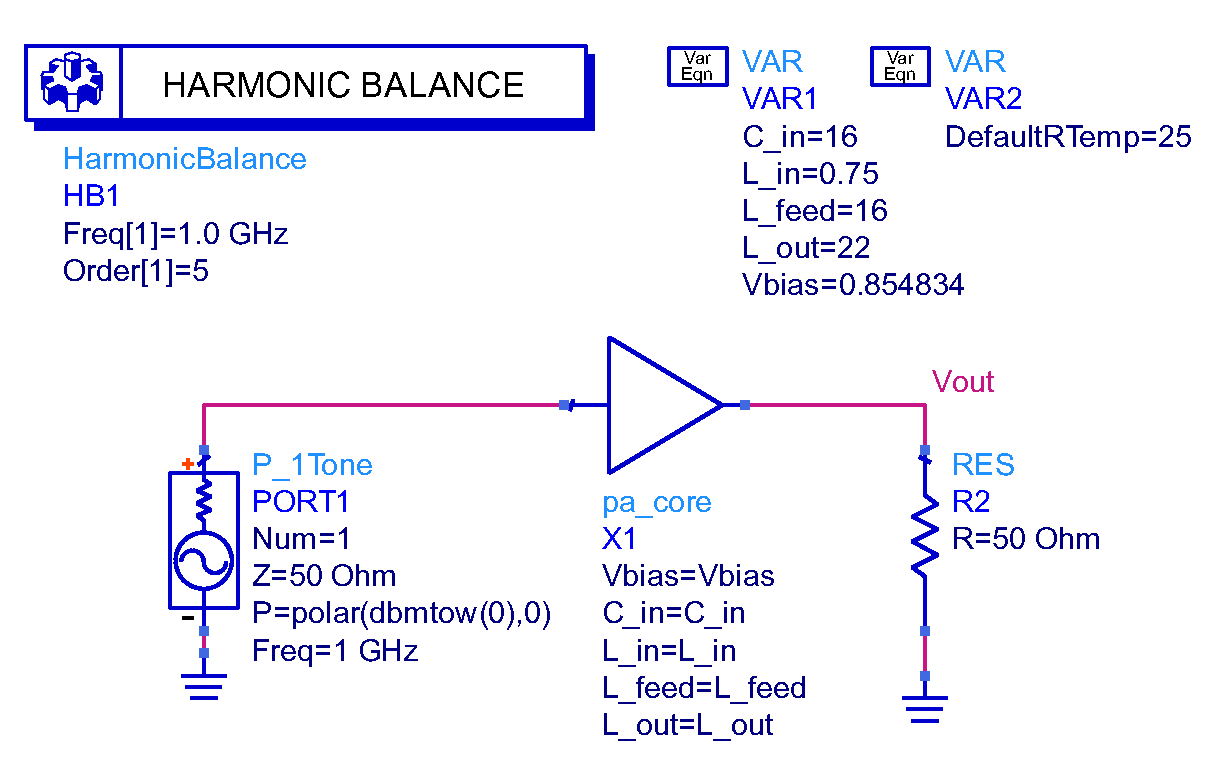
\includegraphics[width=0.85\textwidth]{Figures/2_PA/PA_OUTPUT_SPECTRUM_circuit.pdf}
\captionsetup{justification=centering}
\caption{Esquemático de verificación del PA para \\ análisis de espectro de salida.}
\label{fig:pa_spectrum_circuit}
\end{figure}


La simulación de Balance Armónico se configura con orden 5, lo que permite analizar hasta el quinto armónico de la frecuencia fundamental. La fuente de entrada (\texttt{P\_1Tone}) se configura con una potencia de \qty{0}{\dBm} y una impedancia de \qty{50}{\ohm}.

\subsubsection{Espectro de Salida}

La Figura \ref{fig:pa_output_spectrum} presenta el espectro de potencia a la salida del amplificador para una entrada de \qty{0}{\dBm} a \qty{1}{\GHz}.

\begin{figure}[htbp]
\centering
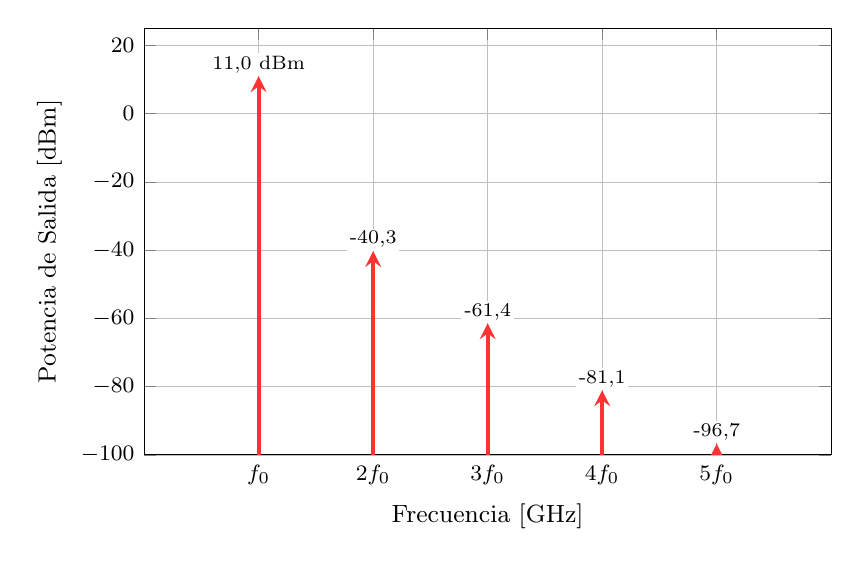
\begin{tikzpicture}
\begin{axis}[
    width=0.85\textwidth,
    height=7cm,
    xlabel={Frecuencia [GHz]},
    ylabel={Potencia de Salida [dBm]},
    xmin=0, xmax=6,
    ymin=-100, ymax=25,
    xtick={1,2,3,4,5},
    xticklabels={$f_0$, $2f_0$, $3f_0$, $4f_0$, $5f_0$},
    grid=both,
    grid style={line width=.1pt, draw=gray!30},
    major grid style={line width=.2pt,draw=gray!50},
    tick label style={font=\footnotesize},
    label style={font=\small},
]
% Componentes espectrales como flechas desde el fondo
\draw[-stealth, red!80, line width=1.5pt] (axis cs:1,-100) -- (axis cs:1,10.97);
\draw[-stealth, red!80, line width=1.5pt] (axis cs:2,-100) -- (axis cs:2,-40.29);
\draw[-stealth, red!80, line width=1.5pt] (axis cs:3,-100) -- (axis cs:3,-61.43);
\draw[-stealth, red!80, line width=1.5pt] (axis cs:4,-100) -- (axis cs:4,-81.07);
\draw[-stealth, red!80, line width=1.5pt] (axis cs:5,-100) -- (axis cs:5,-96.74);

% Etiquetas de valores con fondo blanco
\node[above, font=\scriptsize, fill=white, inner sep=1pt] at (axis cs:1,10.97) {11,0 dBm};
\node[above, font=\scriptsize, fill=white, inner sep=1pt] at (axis cs:2,-40.29) {-40,3};
\node[above, font=\scriptsize, fill=white, inner sep=1pt] at (axis cs:3,-61.43) {-61,4};
\node[above, font=\scriptsize, fill=white, inner sep=1pt] at (axis cs:4,-81.07) {-81,1};
\node[above, font=\scriptsize, fill=white, inner sep=1pt] at (axis cs:5,-96.74) {-96,7};

\end{axis}
\end{tikzpicture}
\captionsetup{justification=centering}
\caption{Espectro de potencia a la salida del PA \\ con entrada de 0 dBm a 1 GHz.}
\label{fig:pa_output_spectrum}
\end{figure}

Los resultados muestran:

\begin{itemize}
    \item \textbf{Fundamental (\qty{1}{\GHz}):} $P_{out} = \qty{10,97}{\dBm}$, correspondiente a una ganancia de \qty{10,97}{\dB} para una entrada de \qty{0}{\dBm}.
    \item \textbf{Segundo armónico (\qty{2}{\GHz}):} \qty{-40,29}{\dBm}, aproximadamente \qty{51}{\dB} por debajo del fundamental.
    \item \textbf{Tercer armónico (\qty{3}{\GHz}):} \qty{-61,43}{\dBm}, aproximadamente \qty{72}{\dB} por debajo del fundamental.
    \item \textbf{Armónicos superiores:} Por debajo de \qty{-80}{\dBm}, despreciables.
\end{itemize}

\subsubsection{Distorsión Armónica Total (THD)}

La Distorsión Armónica Total se calcula a partir de la relación entre la potencia de los armónicos y la potencia de la fundamental:

\begin{equation}
THD = \sqrt{\frac{P_2 + P_3 + P_4 + P_5}{P_1}} \times 100\%
\end{equation}

Convirtiendo los valores de dBm a potencia lineal:

\begin{align}
P_1 &= 10^{10{,}97/10} = \qty{12,50}{\mW} \nonumber \\
P_2 &= 10^{-40{,}29/10} = \qty{9,35e-5}{\mW} \nonumber \\
P_3 &= 10^{-61{,}43/10} = \qty{7,19e-7}{\mW} \nonumber \\
P_4 &= 10^{-81{,}07/10} = \qty{7,81e-9}{\mW} \nonumber \\
P_5 &= 10^{-96{,}74/10} = \qty{2,12e-10}{\mW}
\end{align}

Sustituyendo en la ecuación:

\begin{equation}
THD = \sqrt{\frac{9.35 \times 10^{-5}}{12.50}} \times 100\% \approx \mathbf{0.27\%}
\end{equation}

Este valor de THD es equivalente a aproximadamente \qty{-51}{\dB} respecto al fundamental, lo cual es aceptable para aplicaciones de radar donde la pureza espectral moderada es suficiente.

\subsubsection{Resumen del Rendimiento Final}

La Tabla \ref{tab:pa_performance_summary} resume las características de rendimiento del amplificador de potencia optimizado.

\begin{table}[htbp]
\centering
\small
\caption{Resumen del rendimiento del PA optimizado.}
\label{tab:pa_performance_summary}
\begin{tabular}{@{}lcc@{}}
\toprule
\textbf{Parámetro} & \textbf{Valor} & \textbf{Unidad} \\
\midrule
Frecuencia central        & \num{1,0}    & \unit{\GHz} \\
Potencia de entrada       & \num{0}      & \unit{\dBm} \\
Potencia de salida        & \num{10,97}  & \unit{\dBm} \\
Ganancia                  & \num{10,97}  & \unit{\dB} \\
$S_{11}$ @ \qty{1}{\GHz}          & $< \num{-25}$ & \unit{\dB} \\
$S_{22}$ @ \qty{1}{\GHz}          & $< \num{-16}$ & \unit{\dB} \\
THD                       & \num{0,27}   & \unit{\percent} \\
2do Armónico (supresión)  & $\num{-51}$  & \unit{\dBc} \\
\bottomrule
\end{tabular}
\end{table}

Este análisis espectral marca el fin de la síntesis del circuito. El diseño ha evolucionado desde la nota de aplicación de referencia hasta un amplificador personalizado y optimizado para \qty{1}{\GHz}, con parámetros de polarización precisos y rendimiento validado.

\section{Conclusiones}

Contenido pendiente.
